The aim of this short section is to present the various domains of studies seen in this work and explain concepts that are necessary for comprehension. 

\section{LiDAR}
\gls{lidar} is a method for accurately measuring distances and stands for "\textit{light detection and ranging}". \gls{lidar} is used to make high resolution depth maps, and has seen uses in geography, seismology, forestry ... Along with Archaeology. \gls{lidar} has also been in use in some autonomous vehicles. \gls{lidar} is able to map out large regions of terrain and produces very high resolution data, while being relatively cheap. In essence, \gls{lidar} accurately captures the distance between the sensor and an object, similar in how a sonar works. 

In Archaeology, \gls{lidar} is used to create \gls{dem}, that are then integrated into \gls{gis} for analysis. By carefully choosing the wavelength used, \gls{lidar} is able to see through vegetation and show structure that would be otherwise hidden. This makes it a very valuable tool for Archaeology. 

\gls{lidar} works by emitting short laser pulses and measuring the time of flight between its emission and the time at which it hits an object.  

\section{Archaeology Structures}

\section{Deep Learning}\label{overfit}
Deep Learning is a ensemble of techniques which are based on Artificial Neural Networks, with multiple layers stacked upon each other. Those layers will progressively extract higher level features from the input. 

One of the most successful innovation of Deep Learning would be Convolutional Neural Networks, or \gls{cnn}, first introduced by Yann LeCun\cite{lecun98}. Convolution Neurons applies a convolution operation on its input. The matrix that is convoluted is learned through training. \glspl{cnn} are commonly used with images, but have also seen uses in audio signal processing. 

\glspl{cnn} had massive success during the 2010's, where the use of \acrpl{gpu} allowed for a massive increase in computation speed which rendered the use of deeper and more powerful network possible. One of the first of such network was AlexNet\cite{alexNet} which was trained on a commercial \acr{gpu} and outperformed competitors by more than 10 points. Other quickly followed suit, with deeper and more performant nets being developed each year, like GoogleNet\cite{googleNet}, VGG\cite{vgg} and resNet\cite{resNet} which introduced the idea of feature fusion via residual unit. Today, deep convolutional networks with residual units are a staple in computer vision, but are also used in audio analysis\cite{PiczakCNN}\cite{Adavanne_CRNN}\cite{KaoAlRCRNN}\cite{CakirCRNN}\cite{PhanAl_CNN} among various other field with great success.

The work here centers around the task of object detection. This task is actually two fold: given an input image, localise an object then give a classification of this object. A good object detector must be able to do both, but they are evaluated differently. 

A Deep Learning model is trained on a dataset. Deep Learning requires very large amounts of data to correctly train as they are very prone to overfitting. In statistics, a model is said to overfit when it "describes features that arises from noise or variance in the data, rather than the underlying distribution from which the data is drawn"\cite{Webb2010}. In other words, this means that the model has "memorised" the data, and will perform badly on data which it has never seen before. In Figure~\ref{fig:overfit}, we see a classification task where a curve has to be drawn to differentiate two class and the green line is overfitted to the data, while the black line is a more reasonable fit.

Overfitting is an issue that affects all Deep Learning models, but a lot of effort has been done to address this, either by creating a more diverse and robust dataset with data augmentation, or by modifying the network itself via regularisation and normalisation. 

\begin{figure}[h!]
  \centering
  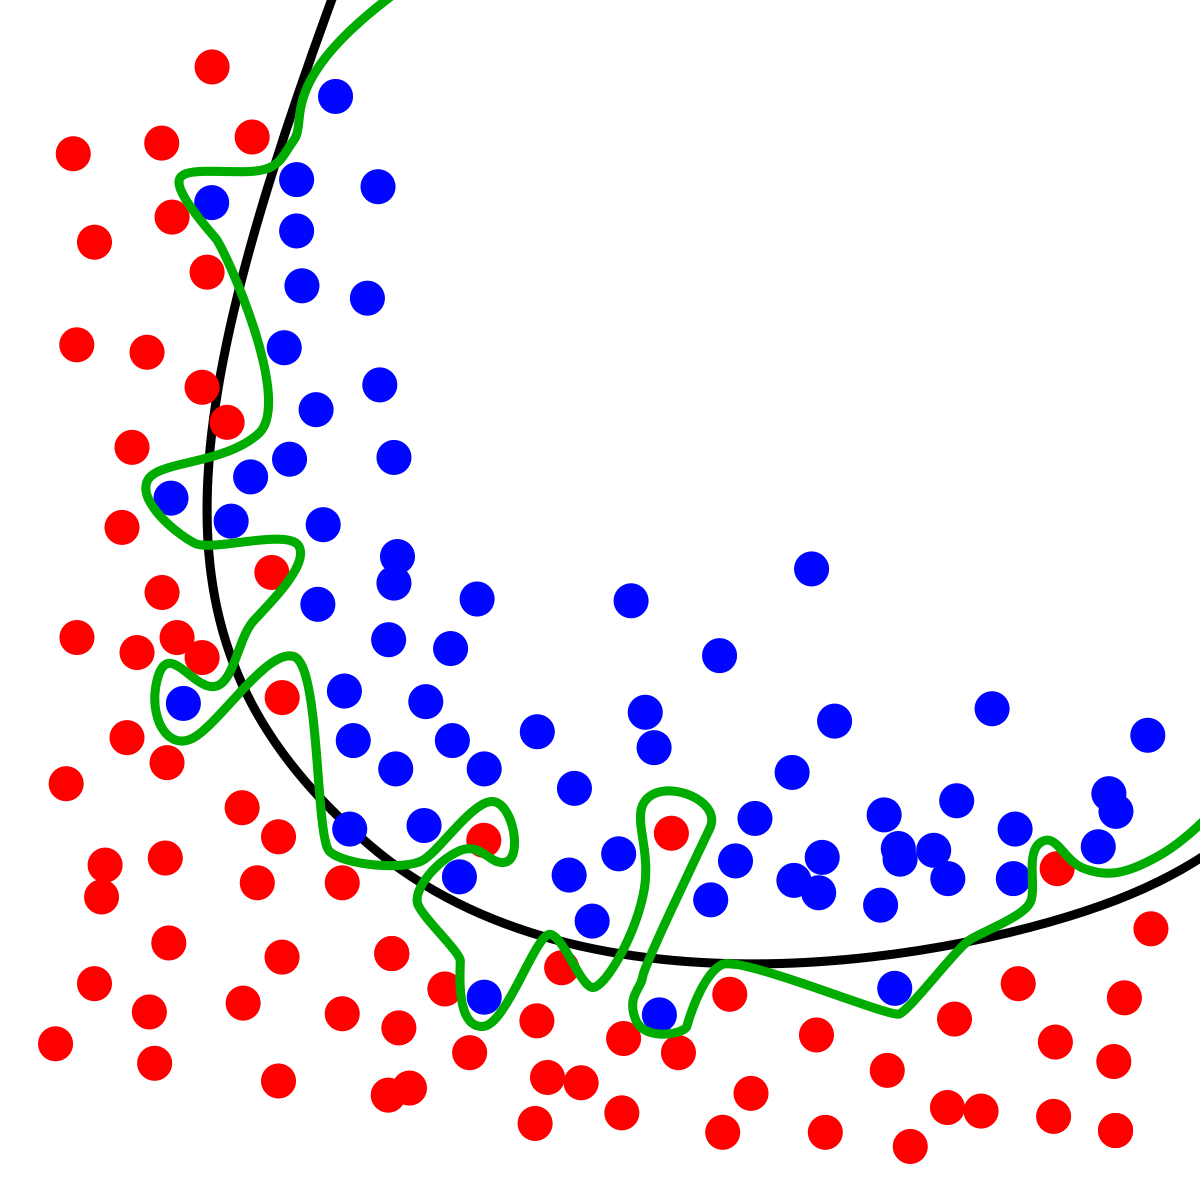
\includegraphics[width=0.5\textwidth]{overfitting}
	\caption[Example of overfitting on a classification task]{Example of overfitting on a classification task. The black line represents a good fit to the data, with an acceptable error rate or, misclassified data points. The green represents an overfit: while the error rate is lower than the black line, the fit is too complicated, and will badly generalize on unseen data. Doc. Wikipedia}
  \label{fig:overfit}
\end{figure}

There are two main parts of training a model on a particular dataset. First the dataset is divided in two sub dataset. One is used for training, and the other for evaluation. For simplicity, we will use an example of classification of an input image. During training, the model will produce a inference based on the input data \textit{i.e.} a label. We will compare the inferred label to the ground truth using a particular metric, like Categorical Cross-Entropy or \gls{mse} and obtain a distance between the two labels. This distance is known as the loss. We will try to reduce the loss by optimising the \gls{weights} of the model using gradient descent, as shown on Figure~\ref{fig:gradDesc}. 

Given a multi variable differentiable function $F(x)$ that is defined in the neighborhood of a point $a \in \mathbb{R}^n$, the gradient descent is defined as follows:
\begin{equation}
	a_{n+1} = a_n - \gamma \nabla F(a_n)
\end{equation}

With a small $\gamma \in \mathbb{R}_+$, we have $F(a_{n+1}) \leq F(a_n)$, meaning that $\gamma \nable F(a)$ is subtracted from $a$, moving toward a minimum. The parameter $\gamma$ is called the learning rate. A large learning rate will mean that the descent might converge faster, but might "overshoot" and miss the minimum, while a small learning rate means a more precise convergence, but will dramatically increase the number of steps necessary. On Figure~\ref{fig:gradDesc}, the learning represent the length of each arrow during the descent. It should be noted that nowadays, gradient descent is rarely used with modern networks, as most uses other optimizers, such as ADAM\cite{AdamOpti} or ADAGRAD\cite{adagrad}.

\begin{figure}[h!]
  \centering
  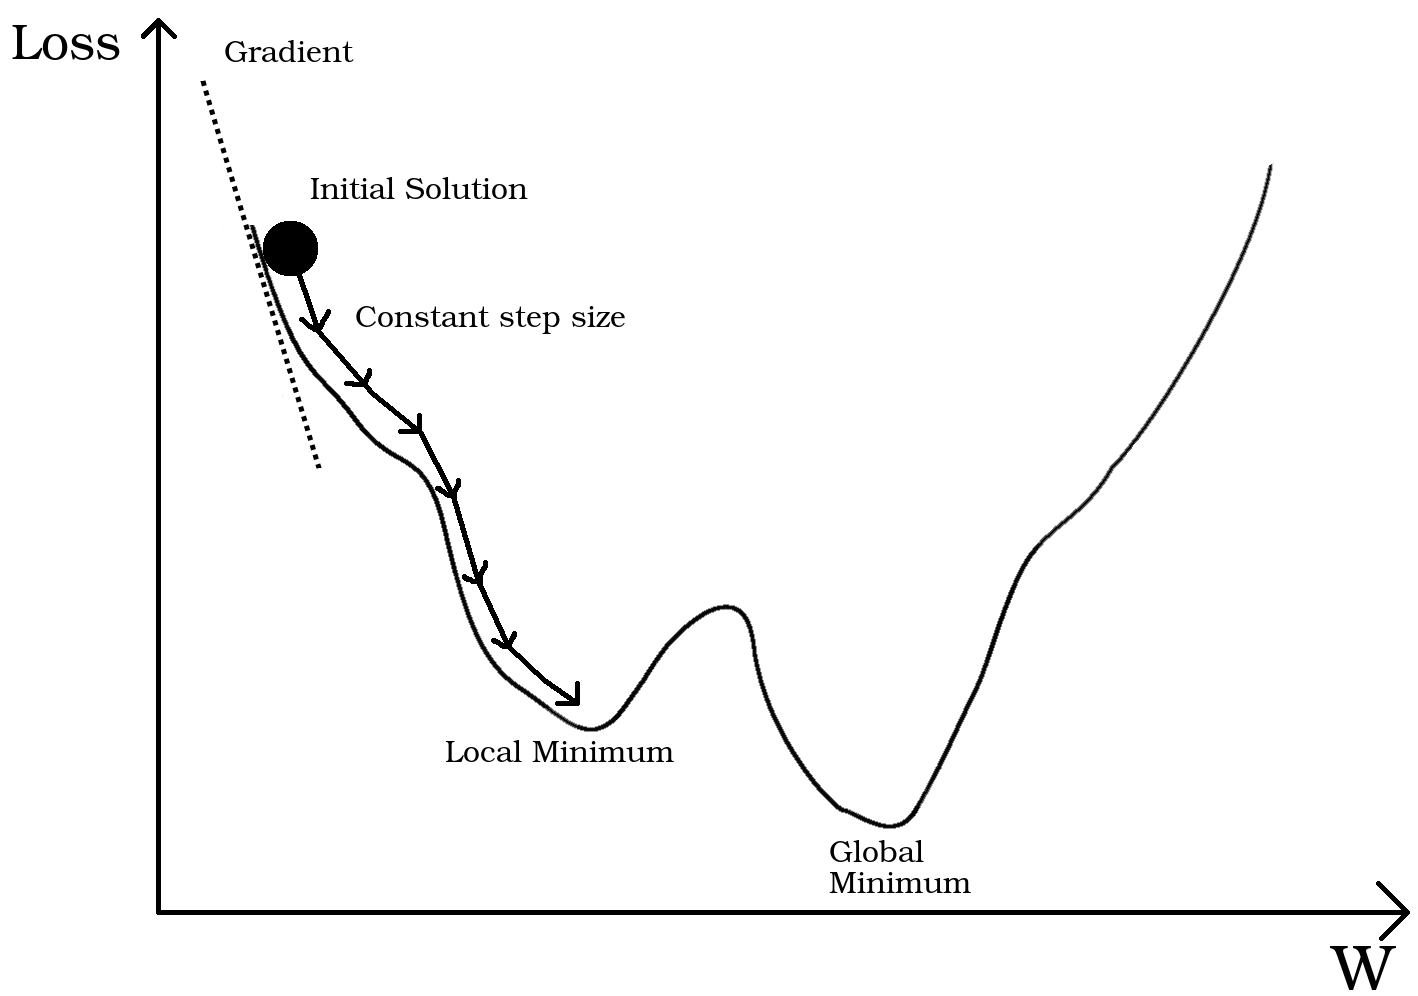
\includegraphics[width=0.7\textwidth]{gradDescent}
	\caption[Gradient Descent]{Gradient Descent on a loss function with one parameter. Since the loss function of neural network is not convex, there are possibly multiple minimum, which the gradient descent algorithm can get "stuck" into. As the dimensionality of the problem increase, the complexity of the dynamics of the gradient descent increase.}
  \label{fig:gradDesc}
\end{figure}

Since the gradient gives the direction of steepest incline of a differentiable function $F(x)$, this means that the function $F(x)$ declines the fastest in the direction of negative gradient. In Deep Learning backpropagation is used, an recursive and efficient process that is able to compute the gradient with respect to the weight of the network.

